\section{Simulation Analysis}
\label{simulanal}


In this section of our report, we are going to simulate the modeled circuit using NGspice. Our main objective with this simulation is confirming the validity of our theoretical approach and try to explain any major discrepancies. We are particularly interested in the merit figure value, as it measures how well our circuit completes the task of amplifying the audio. 

First of all, it's important to analyse and ensure the transistors are working in the desired region as, otherwise, none of our predictions would be validated.
First of all, taking a look at the NPN transistor, which is present on the gain stage, the condition for operating on the forward active region is that $V_{CE}>V_{BE}$. In the simulation, we obtained the following results:

\begin{table}[h]
\centering
\begin{tabularx}{0.6\textwidth} {
  | >{\raggedright\arraybackslash}X
  | >{\raggedleft\arraybackslash}X | }
 \hline
Vce & 4.92668 V\\ \hline
Vbe & 0.654762 V\\ \hline
Correct F.A.R\\ \hline

\end{tabularx}
\caption{NPN transistor in forward active region}
\end{table}

On the other hand, for the PNP transistor, present on the ouput stage, the condition for operating in the forward active region is $V_{EC}>V_{EB}$. In the simulation, we obtained the following results:

\begin{table}[H]
\centering
\begin{tabularx}{0.6\textwidth} {
  | >{\raggedright\arraybackslash}X
  | >{\raggedleft\arraybackslash}X | }
 \hline
Vec & 5.77796 V\\ \hline
Veb & 0.70695 V\\ \hline
Correct F.A.R & yes\\ \hline

\end{tabularx}
\caption{PNP transistor in forward active region}
\end{table}
Now it's important to analyse certain components of the circuit to fully understand their functioning.

\subsection{Coupling Capacitors}

\par 


As previously explained, the coupling capacitors are responsible for blocking the DC signal, as we only want to amplify the AC signal. The DC block is especially important, because it could imply that the transistor isn't always in the forward active region. Taking a look at the capacitor impedance formula, $\frac{1}{jwc}$, if the frequency is equal to zero, the impedance will be infinite, and therefore it will act as an open circuit. We've seen on classes that higher capacitances, lead to lower cut-off frequencies, and larger bandwidths. We were able to witness this on the simulation. 


\subsection{Bypass Capacitors}

\par 
The main functionality of the bypass capacitor is to allow almost all current to flow through, since it will have a really low impedance for medium-high frequency. This capacitor was needed in this circuit, since the presence of the $R_E$ resistor, took a significant toll on the gain value. The $R_E$ resistor could not be removed since it has the important function of diminishing the temperature effect in the DC voltage.
 

\subsection{Resistor $R_C$}

\par Lastly, it's important to address the way resistor $R_C$ impacts the gain. As the gain and $R_C$ are proportional, the higher the resistor value, the higher the gain and consequently, the merit.

%--VER MELHOR R_C
Finally, the effect of $R_C$ on the circuit gain is important to be studied. As the gain is proportional to the value of $R_C$, the higher $R_C$ is, the higher the gain will be and thus the merit.   

\subsection{Impedances Analysis}

Now, we will take a look at the output and input impedances, which are computed in the tables below:


\begin{table}[H]
\centering
\begin{tabularx}{0.6\textwidth} {
  | >{\raggedright\arraybackslash}X
  | >{\raggedleft\arraybackslash}X | }
 \hline
Zin & -1445.55 + 303.662 j\\ \hline

\end{tabularx}
\caption{Input impedance in Ohm}
\end{table}

\begin{table}[H]
\centering
\begin{tabularx}{0.6\textwidth} {
  | >{\raggedright\arraybackslash}X
  | >{\raggedleft\arraybackslash}X | }
 \hline
Zo & 25.8525 + 1.29181 j\\ \hline
Zo(int) & 25.8848\\ \hline

\end{tabularx}
\caption{Output impedance in Ohm}
\end{table}
As previously explained, when looking at the impedances, we expect the impedance seen by the input voltage generator to be really high, in order to minimize the voltage drop due to the internal resistance of the voltage generator (following the voltage divider formula). On the other hand, when looking at the output impedance, we expect it to be really low, so the load resistor takes almost full advantage of the voltage, when looking at the voltage divider formula. As you can see in the table above, the output impedance is still quite high when compared to the 8 Ohm load resistor. This is due to the optimal merit value obtained in our Matlab optimization.



\subsection{Merit Figure}

Finally, after explaining our thought process and the way components impacted our circuit, let's take a look at the merit figure, as well as all the important values that should be taken in consideration in its calculation.

\begin{table}[H]
\centering
\begin{tabularx}{0.6\textwidth} {
  | >{\raggedright\arraybackslash}X
  | >{\raggedleft\arraybackslash}X | }
 \hline
VGain & 34.1403\\ \hline
Bandwidth & 1.22339E+06 Hz\\ \hline
LowerCutoffFreq & 15.8089 Hz\\ \hline
HigherCutoffFreq & 1.22341E+06 Hz\\ \hline
Cost & 2198.94\\ \hline
merit & 1201.48\\ \hline

\end{tabularx}
\caption{Simulation results}
\end{table}
\subsection{Comparison between Theoretical and Simulation Analysis}

Even though we are pretty satisfied with our simulation results, it is important to note that are some discrepancies between the theoretical and the simulation analysis. This could be due to some errors associated with the theoretical model used, when compared to the "real" one in NGspice.

\begin{figure}[H]\centering
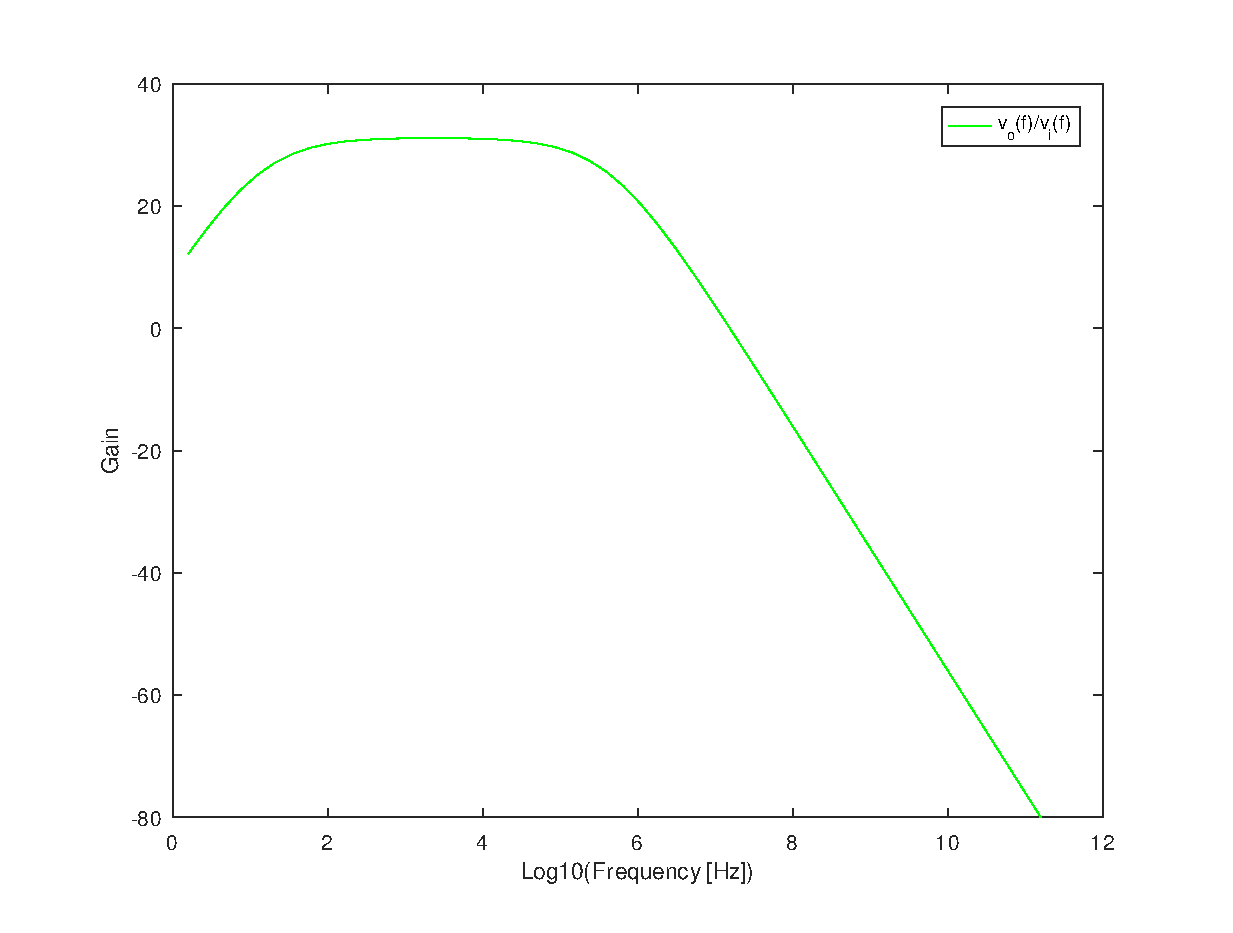
\includegraphics[width=0.7\linewidth]{grafico_octave.eps}
\caption{Theoretical Output Voltage}
\label{fig:snat}
\end{figure}


\begin{figure}[H]\centering
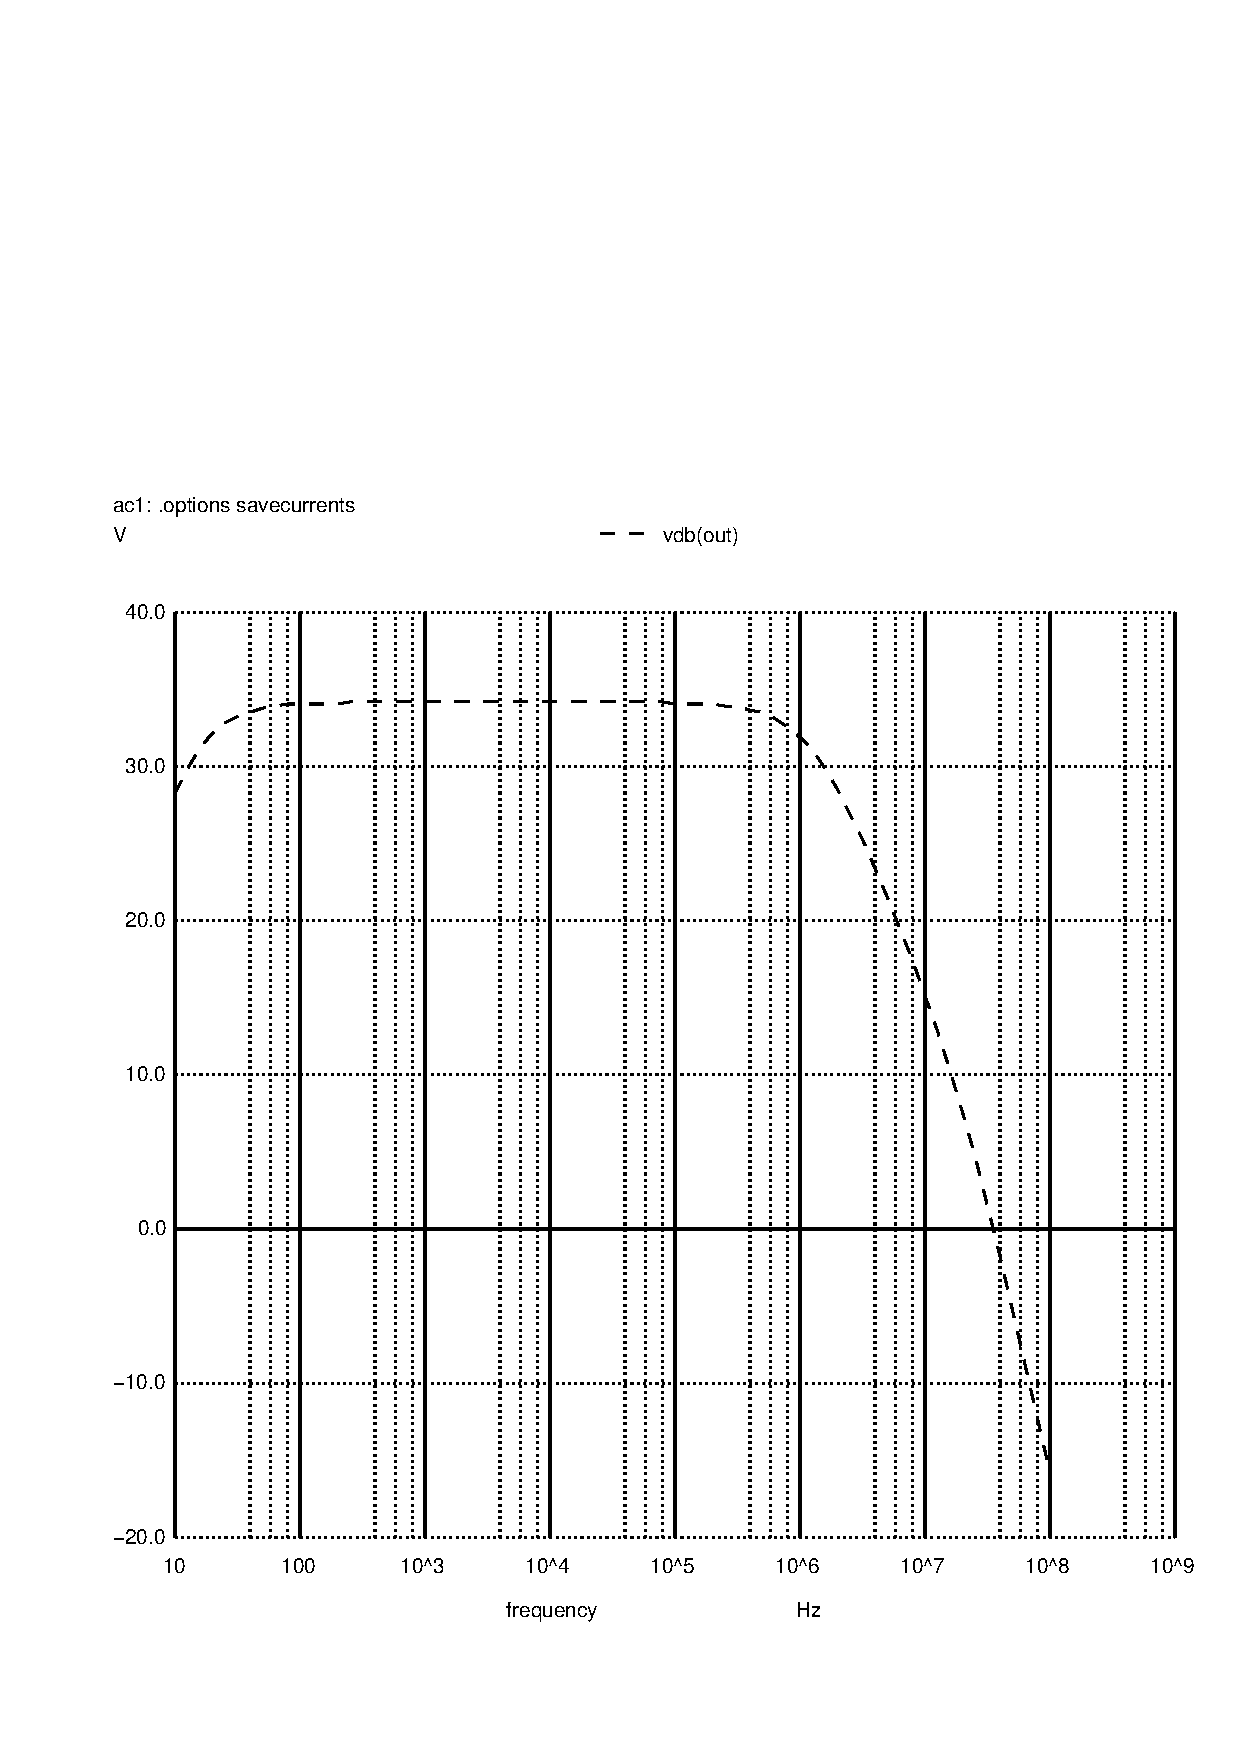
\includegraphics[width=0.7\linewidth]{vo2f.pdf}
\caption{Simulation Output Voltage}
\label{fig:snat}
\end{figure}

Looking at both graphics, we can testify that the prediction of our theoretical model is accurate, in comparison to the simulation.
